\section{Integration und Programmierung der Steuerungstechnik \textcolor{gray}{ (Vincent Sonvilla)}}


\subsection{Aufgabenstellung}


\subsection{Tia-Portal Grundlagen}

Tia Portal (Totally Integrated Automation Portal) ist die zentrale Software von Siemens zur Programmierung, Konfiguration und Diagnose von Automatisierungssystemen. Es ermöglicht die Steuerung von SPS (Speicherprogrammierbare Steuerungen), HMI (Bedienpanels) und Antrieben in einer einzigen Umgebung. Alle folgenden Informationen, sowie Anwendungen beziehen sich auf die genutzte Tia Portal Version (V18) sowie Hardware (S7-1513).

    \subsubsection{Allgemeines}

        \paragraph{Arbeitsweise einer SPS} \mbox{} \\
        Eine SPS arbeitet zyklisch. In Abb. \ref{Arbeitsweise_einer_SPS} wird gezeigt wie ein solcher Zyklus aussieht. Bei erstmaligem Starten oder Neustarten der SPS werden zuerst alle Ausgänge, Merker, etc. auf Null gesetzt. Danach startet die zyklische Arbeitsweise. Zunächst wird ein Prozessabbild der Eingänge gemacht. Mit diesen Eingangswerten wird dann das Programm ausgeführt. Anschließend wird ein Prozessabbild der Ausgänge gemacht. Dieses wird dann an die Ausgänge übergeben. Danach beginnt der Zyklus von vorne. (vgl.\cite{Arbeitsweise_der_SPS})
        \begin{figure}[H]
            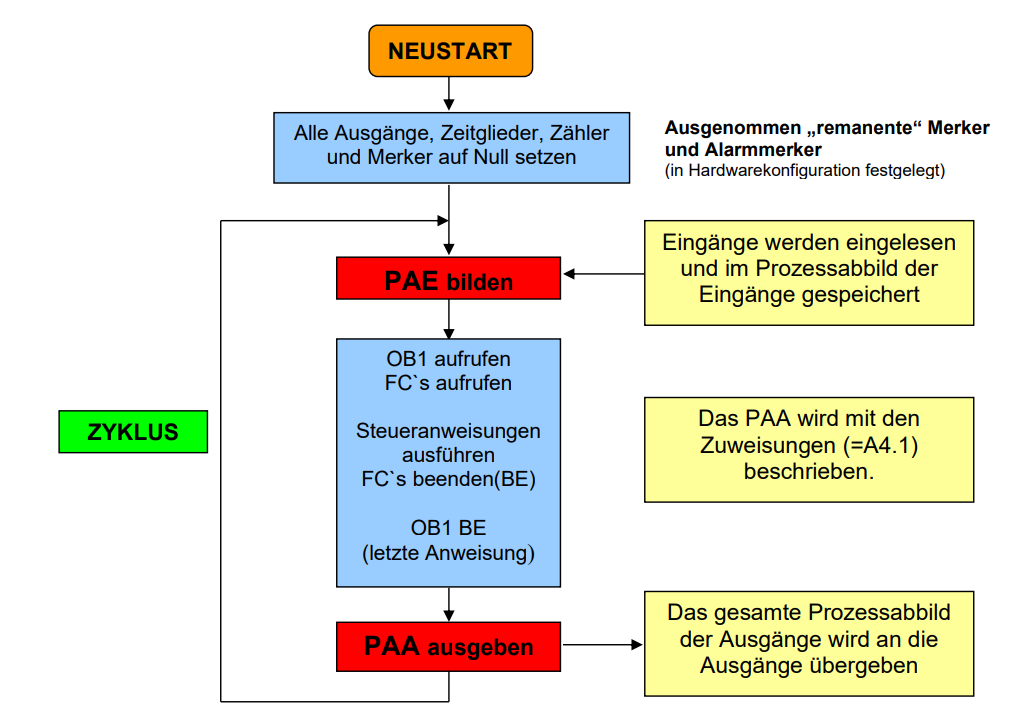
\includegraphics[width=0.9\textwidth]{Sonne/Arbeitsweise_einer_SPS.png}
            \caption{Arbeitsweise einer SPS, Quelle: \cite{Arbeitsweise_der_SPS}}
            \label{Arbeitsweise_einer_SPS}
        \end{figure}


    \subsubsection[Programmbausteine]
    {Programmbausteine}
    
    In Tia Portal werden Programmbausteine genutzt, um Steuerungsprogramme modular und strukturiert zu gestalten. Dadurch werden Programme übersichtlicher, wiederverwendbar und effizienter. Es gibt unterschiedliche Arten von Programmierbausteinen:

    \begin{itemize}
        \item[1.] \textbf{OB(Organisationsbausteine)} \\
            Organisationsbausteine werden verwendet um das Anwenderprogramm hierarchisch zu strukturieren. Auch für OBs stehen,wie in Abb. \ref{Organisationsbausteine} gezeigt, unterchiedliche Bausteine zur Verfügung:
            \begin{figure}[h]
                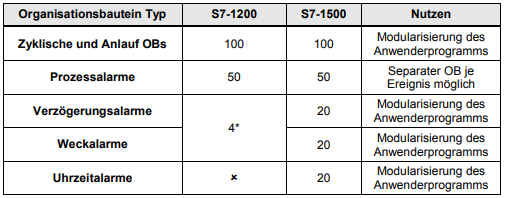
\includegraphics[width=\textwidth]{Sonne/Tia-Portal_Organisationsbausteine.png}
                \caption{Organisationsbausteine, Quelle: \cite{Programmierleitfaden_für_S7-1500}}
                \label{Organisationsbausteine}
            \end{figure}

            Organisationsbausteine steuern unterschiedliche Vorgänge:
            \begin{itemize}
                \item Anlaufverhalten der Steuerung
                \item Zyklische Programmbearbeitung
                \item Alarmgesteuerte Programmbearbeitung
                \item Behandlung von Fehlern
            \end{itemize}
            Werden in einem Programm mehrere OBs aufgerufen, so werden die OBs in aufsteigender Reihenfolge der OB-Nummer abgearbeitet. 

        \item[2.] \textbf{FC (Funktionen)} \\
            Funktion haben keinen zyklischen Datenspeicher, deswegen können Bausteinparameter nicht bis zum nächsten Aufruf gespeichert werden. Daher müssen Funktionen bei jedem Aufruf mit Aktualparametern versorgt werden. Um kein zufälliges Verhalten enstehen zu lassen sind die Werte immer mit einem Standardwert vorbelegt. Will man die Daten einer Funktion dauerhaft speichern, so muss ein globaler Datenbaustein verwendet werden.\\
            Funktionen werden eingesetzt, um häufig wiederkehrende Anwendungen durchzuführen.
            
        \item[3.] \textbf{FB (Funktionsbausteine)} \\
            Im Gegensatz zu Funktionen haben Funktionsbausteine einen zyklischen Datenspeicher -Instanz DB-, in welchem Werte dauerhaft gespeichert werden. Dadurch behalten statische Variablen ihren Wert von Zyklus zu Zyklus. Wie bei Funktionen sind die Werte mit einem Defaultwert vorbelegt.\\
            Funktionsbausteine können genutzt werden, um Unterprogramme für unterschiedliche Anwendungen zu erstellen. Dies erleichtert das Strukturieren eines Anwenderprogramms. Bei mehrfacher Verwendung von Funktionsbausteinen empfiehlt sich die Verwendung von Multiinstanz-DBs (siehe 6.Multiinstanzen).
        
        \item[4.] \textbf{Global-DB (Datenbausteine)} \\
            Globale Datenbausteine speichern variable Daten, die dem kompletten Programm zur Verfügung stehen. Wie in Abb.\ref{Zugriff auf Global-DB} ersichtlich, bedeutet das ,dass alle Bausteine Zugriff auf den Global-DB haben.

            \begin{figure}[h]
                \centering
                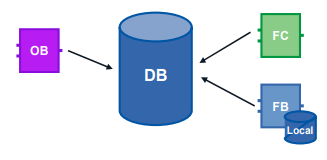
\includegraphics{Sonne/Zugriff_auf_Global-DBs.png}
                \caption{Zugriff auf Global-DB, Quelle \cite{Programmierleitfaden_für_S7-1500}}
                \label{Zugriff auf Global-DB}
            \end{figure}

            In Globalen Datanbausteinen können jegliche Datentypen genutzt werden.\\
            Globale DBs werden verwendet, wenn Daten in verschiedenen Programmteilen bzw. Bausteinen benötigt werden.

        \item[5.] \textbf{Instanzen} \\
            Wird ein Funktionsbaustein aufgerufen, so nennt man das Instanz. Die Daten der Instanz, werden im sogenannten Instanzdatenbaustein gespeichert. Instanz-DBs werden automatisch nach den Vorgaben des Funktionsbausteins erzeugt und können somit nicht direkt geändert werden. Der Instanz-DB hat einen dauerhaften Speicher, welcher die Schnittstellen Input, Output, InOut sowie Static beihaltet. Zusätzlich besitzt der Instanz-DB einen flüchtigen Datenspeicher in dem temporäre Variablen gespeichert werden. Diese sind dadurch immer nur für einen Zyklus gültig.
            
        \item[6.] \textbf{Multiinstanzen} \\
            Bei Multiinstanzen speichert der Funktionsbaustein seine Daten in den Instanz-DB des übergeordneten Funktionsbaustein. Das heißt es wird in einem FB ein anderer FB aufgerufen. Dieser speichert seine Daten dann im Instanz-DB des Funktionsbausteins, welcher ihn aufgerufen hat. Multiinstanzen helfen das Programm übersichtlicher sowie strukturierter zu halten, da man mehrere Instanzen in einer einzigen vereint.
            

    \end{itemize}
    (vgl. \cite{Programmierleitfaden_für_S7-1500})

    \subsubsection[Technologieobjekte]{Technologieobjekte}
    Technologieobjekte dienen dazu die Ansteuerung und Handhabung von technischen Funktionen, insbesondere von Motoren, Achsen, etc. zu vereinfachen. Es existieren eine Vielzahl an unterschiedlichen Technologieobjekten. In nachfolgenden Absätzen werden die für das Projekt relevanten Technologieobjekte genauer erklärt.

    \begin{itemize}

        \item[1.] \textbf{Positionierachse (PositioningAxis)} \\
            Dieses Technologieobjekt dient zur genauen Positionierung einer Achse, sowie der Rückmeldung der aktuellen Achsposition. Zusätzlich wird die Zielposition automatisch gehalten. \\
            Für die Positionierachse stehen folgende Motion Control Anweisungen zur Verfügung: 
            \begin{itemize}
                \item Home \\
                    \subitem Aktives oder passives Referenzieren der Achse.
                \item MoveAbsolut \\
                    \subitem Fahren der Achse auf eine absolute Position.
                \item MoveRelativ \\
                    \subitem Fahren der Achse auf eine Position relativ zur aktuellen Position.
                \item MoveSuperimposed \\
                    \subitem Starten einer überlagerten Bewegung zu einer bereits laufenden Bewegung.
                \item TorqueLimiting \\
                    \subitem Aktivieren einer Momentbegrenzung oder Festanschlagserkennung.
                \item SetSensor \\
                    \subitem Umschalten des Gebers für die Achse. 
            \end{itemize}
            

        \item[2.] \textbf{Gleichlaufachse (SynchronousAxis)} \\
            Das Technologieobjekt Gleichlaufachse enthält alle Funktionen des Technologieobjekts Positionierachse. Zusätzlich lässt sich die Achse mit einer Leitachse verschalten, sodass diese der Positionsänderung der Leitachse folgt. Dieses Technologieobjekt wird verwendet um synchrone bzw. positionsabhängige Bearbeitungsvorgänge auszuführen. \\
            Der Gleichlaufachse stehen folgende zusätzliche Motion Control Anweisungen zur Verfügung:
            \begin{itemize}
                \item GearIn \\
                    Starten eines relativen Gleichlaufs einer Leit- und Folgeachse.
                \item GearInPos \\
                    Starten eines absoluten Gleichlaufs einer Leit- und Folgeachse unter Vorgabe einer Synchronposition.
                \item PhasingAbsolut \\
                    Absolutes Verschieben des Leitwertbezugs während eines aktiven Gleichlaufs.
                \item PhasingRelativ \\
                    Relatives Verschieben des Leitwertbezugs während eines aktiven Gleichlaufs.
                \item CamIn \\
                    Start eines absoluten Kurvenscheibengleichlaufs.
                \item SynchronizedMotionSimulation \\
                    Simulation eines aktiven Gleichlaufs. 
            \end{itemize}
             (vgl. \cite{Technologieobjekte})
    \end{itemize}

    \subsubsection{Programmiersprachen}
    In Tia Portal stehen unterschidiedliche Programmiersprachen zu Verfügung. Je nach Präferenz bzw. Aufgabe ist das Nutzen der richtigen Sprache von Vorteil. Daher folgt hier eine Auflistung der möglichen Programmiersprachen, welche sich in textbasierte (tb.) oder graphische (gr.) Sprachen unterteilen. 

    \begin{itemize}
        \item [1.] \textbf{Funktionsplan (FUP), gr.} \\
            FUP ist eine graphisch augebaute Programmiersprache. Sie besteht aus unterschiedlichen Bausteinen, in Blockdarstellung, welche graphisch durch Linien verknüpft werden. Die Signalverarbeitung bei FUP läuft von links nach rechts. Die Programmierlogik in FUP ist übersichtlich und schnell nachzuvollziehen, weswegen diese Sprache für Anfänger relativ gut geeignet ist. 
            (vgl. \cite{Programmiersprachen_der_SPS})

        \item[2.] \textbf{Kontaktplan (KOP), gr.} \\
            Der Kontakplan ähnelt einem Stromlaufplan, der anstatt von oben nach unten von links nach rechts verläuft. Für die Programmierung werden Symoble wie Öffner, Schließer und Ausgänge verwendet. Da nicht für jeden Baustein ein Symbol verfügbar ist, werden solche Bausteine in FUP dargestellt. Der logische Verlauf der Schaltung ist dabei von links nach rechts und von oben nach unten.
            (vgl. \cite{Programmiersprachen_der_SPS})

        \item[3.] \textbf{Anweisungsliste (AWL), tb.}\\
            AWL ist eine textbasierte Programmiersprache, welche an Assembler angelehnt ist. Die Programmiersprache AWL wird hauptsächlich zur logischen Verknüpfung von Ein- und Ausgängen verwendet. In AWL werden Anweisungen in der Reihenfolge geschrieben, in der sie ausgeführt werden sollen. Da AWL für die Programmierung von größeren Projekten eher ungeeignet ist, wird es in neueren Programmen immer weniger verwendet.
            (vgl. \cite{Anweisungsliste})

        \item[4.] \textbf{S7-Graph, gr.} \\
            S7-Graph wird verwendet um Ablaufsteuerungen übersichtlich und schnell zu programmieren. Die zu ausführenden Aktionen werden in unterchiedliche Einzelschritte aufgeteilt. Zwischen diesen Einzelschritten befinden sich Transitionen. Transitionen sind Weiterschaltbedingungen, welche erfüllt werden müssen damit zum nächsten Schritt weitergeschaltet wird. Der Ablauf der Steuerung erfolgt von oben nach unten. 

        \item[5.] \textbf{Structered Code Language (SCL), tb.} \\
            SCL ist eine höhere Programmiersprache, welche sich an Pascal orientiert. SCL ist für mathematische Funktionen, sowie das Programmieren von Schleifen oder if-Bedingungen besser geeignet als andere Programmiersprachen der SPS. In SCL hat man trotzdem Zugriff auf die typischen Elemente einer SPS, wie Eingänge, Ausgänge, Zeiten, Merker, Bausteinaufrufe und dergleichen.
            (vgl. \cite{SCL})

    \end{itemize}


    \subsubsection{Bilbliotheken } \mbox{}
    In Tia Portal sind nicht alle Funktionen integriert zur welcher die SPS fähig wäre. Deswegen gibt es Bibliotheken, um projektspezifische Funktionen in das Programm zu intergrieren. Bibliotheken können zusätzlich dazu genutzt werden um projektspezifische Bausteine oder Funktionen auch für andere Programme zugänglich zu machen. Generell kann man Bibliotheken in zwei unterschiedliche Arten unterteilen: Projektbibliothek (Project library) und Global Bibliothek (Global library). Projektbibliotheken sind im Projekt integriert und werden im Projekt verwaltet. Dies ermöglicht eine Wiederverwendung von Bausteinen, Funktionen, usw. innerhalb des Programms. Globale Bibliotheken hingegen sind projektunabhängig und können deshalb innerhalb von mehreren Projekten verwendet werden. In Bibliotheken gibt es dann wieder zwei unterschiedliche Möglichkeiten der Ablagerung. Man unterscheidet zwischen Kopiervorlagen (Master copies) und Typen (Types). Elemente, die in \enquote{Kopiervorlagen} gespeichert sind, sind mit dem kopierten Element nicht verbunden. Typen hingegen sind mit ihren Verwendungsstellen im Projekt verbunden. Das heißt, wenn Type verändert werden, wird dies im Projekt automatisch aktualisiert. Im Falle, dass ein Typ gelöscht wird, werden alle Verwendungen automatisch mitgelöscht.  
    (vgl. \cite{Programmierleitfaden_für_S7-1500})


        \paragraph{Einbindung von globalen Bibliotheken} \mbox{} \\
        \label{Bilbliotheken}
        Bibliotheken in Tia Portal hinzuzufügen ist intuitiv und simpel. Der erste Schritt ist das Downloaden der richtigen Bibliothek. Diese können Online auf Websiten, von Siemens oder Drittherstellern, gefunden werden. Um diese jedoch herunterzuladen, braucht man einen dazu berechtigten Siemens-Account. Ist die richtige Bibliothek gefunden und heruntergeladen, erfolgt der zweite Schritt. Zuerst wird Tia Portal geöffnet. Dann geht man auf die Projektansicht. Daraufhin findet man ganz rechts, als vierten Reiter von oben den Punkt Bibliotheken. Klickt an auf diesen erscheint ein Fenster, welches der Höhe nach in zwei Teile aufgeteilt ist. Die obere Hälfte ist für die Projektbibliothek. In der unteren Hälfte findet man die Globalen Bibliotheken. Um nun eine neue Bibliothek einzubinden, klickt man auf das zweite Symbol von links "Globale Bibliothek öffnen". Das Symbol ist ein Buch mit einem grünen Pfeil rechts oben. Jetzt öffnet sich wieder ein Fenster. Hier befindet sich  dann der Ordner, aus dem die zu integrierende Bibliothek ausgewählt wird. Im Anschluss wird die Datei mit dem Datenformat .alxx (xx ... Version Tia-Portal (18)) geöffnet. Nun ist die gewünschte Bibliothek verfügbar. Alle Bausteine die diese Bibliothek zur Verfügung stellt,können nun per Drag-and-Drop ins Programm gezogen werden.
        (vgl. \cite{Bibliotheken})


\subsection{Motoransteuerung}
Eine weitere Hauptaufgabe der SPS ist es, die Ansteuerung der Motoren zu vollziehen. Hierbei stehen die Daten zur Verfügung, welche vom Server geschickt werden. Dies beinhaltet für die Motoransteuerung folgende Aufgaben: Positionsfahren (Ein/Auslagerung), Ansteuerung des Motors des Querförderes sowie die Ansteuerung der Asynchronmaschine des Förderbandes. Bei allen Motoren, bis auf den Motor für das Förderband, handelt es sich um Schrittmotoren. Es werden zwei unterschiedliche Motortypen verwendet: Nema 23 Closed Loop und Nema 17, wobei Nema 23 der stärkere der beiden Motoren ist. Die Nema 23 Motoren werden für das Ansteuern der X- und Y-Achse verwendet. Der Querförderer sowie die Z-Achse über die Nema 17 Motoren. Zu bedenken ist, dass jede Achse von zwei Motoren angetrieben wird und sich daher eine Anzahl von 7 Schrittmotoren plus einen Asynchronmotor ergibt. Für jeden der Schrittmotoren gibt es eine Schrittmotortreiber. Dieser regelt den Motor anhand der Kontrollsignale, die dieser von der SPS bekommt. 

\subsubsection[Kontrollsignale für den Motortreiber]
{Kontrollsignale für den Motortreiber }

Die zwei Hauptsignale die der Treiber von der SPS bekommt, sind ein PTO-Signal sowie ein boolsches Signal, welches für die Drehrichtung verwendet wird (Direktion). Zusätzlich dazu gibt es ein zweites Boolsches Signal für die Freigabe des Motors (Enable). Ein weiteres Signal geht vom Motortreiber aus, nämlich ein Alarmsignal (Alarm). Dieses wird gesendet, wenn der Motortreiber folgende Fehler erfährt: Überspannung, Überstrom, Kurzschluss sowie Positionsschleppfehler.

    \begin{itemize}
        \item [1.] \textbf{Pulse Train Output (PTO)} \\
        Das PTO-Signal besteht aus verschiedenen Pulsen mit Ein- zu Auszeit im Verhältnis 50 : 50 Prozent. Für jeden dieser Pulse bewegt sich der Motor um einen Schritt. Wie groß dieser Schritt ist hängt davon ab, wie viele Schritte benötigt werden um eine volle Umdrehung des Motors zu vollziehen. Dies kann man am Schrittmotortreiber einstellen. Bei diesem Projekt ist eine Umdrehung des Motors in 1600 Schritte eingeteilt. Das heißt, das PTO Modul schickt 1600 solcher Pulse , damit sich der Motor einmal dreht. Das heißt die SPS regelt die Frequenz mit welcher die Pulse hinausgeschickt werden und somit die Geschwindigkeit des Motors. 

        \item [2.] \textbf{Direktion} \\
        Dieses Signal ist wie bereits erwähnt ein boolsches Signal. Dies bedeutet, dass das Signal nur zwei Zustände besitzt. Entweder HIGH oder LOW. Dieses Signal bestimmt die Richtung, in welche sich der Motor dreht. Entweder im Uhrzeigersinn (CW) oder gegen den Uhrzeigersinn (CCW). Bei einem HIGH Signal dreht der Motor gegen den Uhrzeigersinn und bei einem LOW Signal im Uhrzeigersinn.

        \item [3.] \textbf{Enable} \\
        Hat wie das Direktion-Signal zwei Zustände: HIGH und LOW. Dieses Signal ist jedoch logisch invertiert. Dies bedeutet, dass bei einem HIGH Signal der Motor gesperrt ist. Der Motor ist nur bei einem LOW-Signal freigegeben. 

        \item [4.] \textbf{Alarm} \\
        Ist ebenfalls ein boolsches Signal mit HIGH und LOW. Sobald der Motortreiber oben genannte Probleme erkennt, wird dieses Signal auf HIGH gesetzt. So sieht man auch in der SPS, dass es zu einem Fehler am Motortreiber gekommen ist. 

    \end{itemize}

Um falsche Ausführungen sowie Abweichungen zu vermeiden, müssen die in Abb. \ref{Sequenzdiagramm} gezeigten , Minimal- und Maximalwerte, eingehalten werden. Damit ein Signal als HIGH aufgefasst wird, muss es über \qty{3.5}{\volt} haben. Soll es jedoch als LOW gesehen werden, so muss die Spannung des Signals unter \qty{0.5}{\volt} fallen. Die Periode des PTO Signals muss länger als \qty{5}{\micro\second} sein, um eine sichere Abarbeitung zu garantieren. Auch darf die Pulsweite, sowie die Zeit die der Puls auf LOW ist, nicht unter \qty{2.5}{\micro\second} fallen. Zusätzlich muss das Enable-Signal mindestens \qty{5}{\micro\second} vor dem Direktion Signal und \qty{10}{\micro\second} vor dem PTO Signal am Motortreiber anstehen. Wie in Abb. \ref{Sequenzdiagramm} zu sehen, muss das Direktion-Signal auch mindestens \qty{5}{\micro\second} vor dem PTO Signal ankommen. 

    \begin{figure}[h]
        \centering
        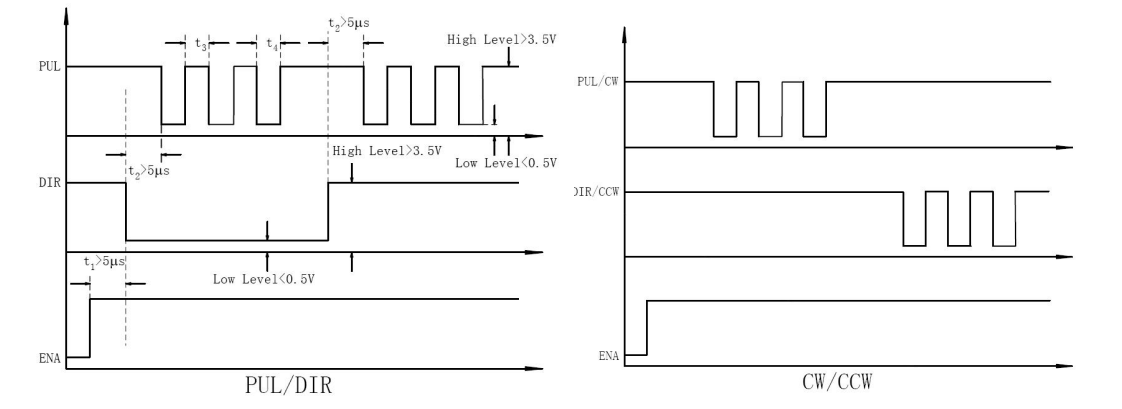
\includegraphics[width = \textwidth]{Sonne/PUL_DIR_ENA-Motor.png}
        \caption{Sequenzdiagramm der Kontrollsignale, Quelle: \cite{User-Manual_CL57T}}
        \label{Sequenzdiagramm}
    \end{figure}

(vgl. \cite{User-Manual_CL57T})

\subsubsection{Motion Control Anweisungen}
Um den Motor in der SPS durch das Programm steuern zu können, wird zuerst das Technologieobjekt für diesen Motor erstellt und mit den richtigen Daten ausgefüllt. Danach ist dieses Technologieobjekt durch Motion Control Anweisungen steuerbar. In den folgenden Abschnitten werden alle für das Projekt relevanten Motion Control Anweisungen erklärt. 

\begin{enumerate}
    \item \textbf{MC\_Power} \\
        Diese Motion Control Anweisung gibt ein Technologieobjekt frei beziehungsweise sperrt es. Wird der Parameter enabel auf HIGH gesetzt, so wird das Technologieobjekt freigegeben. Das Technologieobjekt ist solange freigegeben, solange enable auf HIGH ist. Am Parameter Status kann man dann erkennen, ob das Technologieobjekt freigegeben wurde oder nicht.

    \item \textbf{MC\_Home} \\
        Wird verwendet um eine Achse zu referenzieren. Die Dynamikwerte mit welcher dieser Baustein ausgeführt wird, sind jene, die in der Konfiguration des Technologieobjekts voreingestellt wurden. Es wird unterschiedlich referenziert, je nach dem welcher Wert (0-13) am Parameter Mode anliegt. Ausgeführt wird diese Motion Control Anweisung sobald eine steigende Flanke am Parameter execute erfasst wird. Referenziert ist die Achse erst, wenn der Parameter Done auf HIGH umschaltet. 

    \item \textbf{MC\_MoveAbsolut} \\
        Mit dieser Anweisung wird eine Achse auf eine absolute Position gefahren. Die Parameter Velocity (Geschwindigkeit), Jerk (Ruck), Acceleration (Beschleunigung) und Deceleration (Verzögerung) können bestimmt werden. Werden diese nicht ausgefüllt oder mit einem Wert kleiner null ausgefüllt, so werden die voreingestellten Werte übernommen. Diese Motion Control Anweisung kann nur ausgeführt werden, wenn das Technologieobjekt bereits referenziert ist. Ist das der Fall so wird das Technologieobjekt ausgeführt, wenn es am Parameter execute eine steigende Flanke erkennt. Wenn die Zielposition erreicht wird, schaltet der Paramterer Done auf HIGH. 

    \item \textbf{MC\_GearIn} \\
        Startet einen Getriebegleichlauf zwischen einer Leit- und einer Flogeachse. Dies kann sowohl in Bewegung als auch im Stillstand erfolgen. Als Leitachse können folgende Technologieobjekte ausgewählt werden: Positionierachse, Gleichlaufachse, Externer Geber und Leitachsstellvertreter. Als Folgeachse kann jedoch nur das Technologieobjekt Gleichlaufachse agieren. Der Auftrag wird gestartet sobalb am Parameter execute eine steigende Flanke kommt. Die Snychronisation ist fertiggestellt, wenn der Parameter InGear auf HIGH schaltet.

\end{enumerate}

(vgl. \cite{Tia-Portal_Informationssystem})

\subsubsection{Konfiguration Technologieobjekt}
Um die Technologieojekte nutzen zu können, müssen diese korrekt konfiguriert werden. Das Technologieobjekt für den Nema23 Motor wird wie folgt konfiguriert:

\paragraph{Positionierachse}
    
        \begin{enumerate}
            \item Technologieobjekte
            \item Neues Objekt hinzufügen
            \item Motion Control
            \item TO\_PositioningAxis
            \item Konfiguration
            
                \begin{itemize}

                \item Antrieb $\rightarrow$ Local Modules $\rightarrow$ PTO Modul auszuwählen
                \item Mechanik $\rightarrow$ Spindelsteigung: $= 134,9942$
                \item Dynamik-Voreinstellung: 
                    \subitem Geschwindigkeit:
                        \qty{300}{\milli\meter/\second}
                    \subitem Beschleunigung: 
                        \qty{6000}{\milli\meter/\square\second}
                    \subitem Verzögerung:
                        \qty{6000}{\milli\meter/\square\second}
                \item Positionsgrenzen
                    \subitem HW-Endschalter aktivieren
                    \subitem Variablen wählen
                    \subitem Pegelauswahl: oberer Pegel
                \item Dynamikgrenzen
                    \subitem Geschwindigkeit:
                        \qty{1000}{\milli\meter/\second}
                    \subitem Beschleunigung: 
                        \qty{20000}{\milli\meter/\square\second}
                    \subitem Verzögerung:
                        \qty{20000}{\milli\meter/\square\second}
                \item Referenzieren $\rightarrow$ aktives Referenzieren
                    \subitem Variable wählen
                    \subitem Pegelauswahl: oberer Pegel
                    \subitem Refernzierrichtung: Positiv
                    \subitem Refernziergeschwindigkeit:
                        \qty{25}{\milli\meter/\second}
                
                \end{itemize}
        \end{enumerate}

\paragraph{Gleichlaufachse} \mbox{} \\
Bei der Gleichlaufachse ist bei der Konfiguration ein zusätzlicher Schritt vorzunehmen. Unter Konfiguration - Leitwertverschaltung wird eine Leitwertverschaltung hinzugefügt, in dem man auf \enquote{hinzufügen} klickt und anschließend das Technologieobjekt auswählt, dem die Gleichlaufachse folgen soll.



\subsubsection{Synchronisation}
Die X,Y,Z -Achsen werden von jeweils zwei Motoren angetrieben. Daher müssen die zwei Motoren, welche zusammenarbeiten, synchronisiert werden. Dies wird in der Software, durch die Motion Control Anweisung MC\_GearIn, gelöst. Bei dem Slave muss es sich, wie beschrieben um eine Gleichlaufachse (TO\_SynchronousAxis) handeln. Da die beiden Achsen hardware technisch verbunden sind, muss die Synchronisation im Stillstand erfolgen. Ausgeführt wird die Synchronisation bei einer steigenden Flanke am Parameter Execute. Die Folgeachse bleibt nun solange synchron zur Leitachse, bis es entweder zu einem MC\_GearOut Auftrag kommt, oder die Freigabe der Folgeachse, durch ein LOW Signal am Parameter enable des MC\_Power Bausteins (Folgeachse), nicht mehr vorhanden ist. Ein Sperren der Leitachse über MC\_Power (Leitachse) führt nicht zu einem Synchronisationsverlust. Die voreingestellten Werte bei den Parametern RationNumerator sowie RatioDenominator können übernommen werden. Diese werden nur geändert falls zwischen den zu synchronisierenden Motoren, ein Getriebe vorhanden ist, was bei diesem Projekt jedoch nicht der Fall ist. Ansonsten bleibt der Getriebefaktor bei 1. (siehe Abb. \ref{MC_GearIn})

\begin{figure}[h]
    \centering
    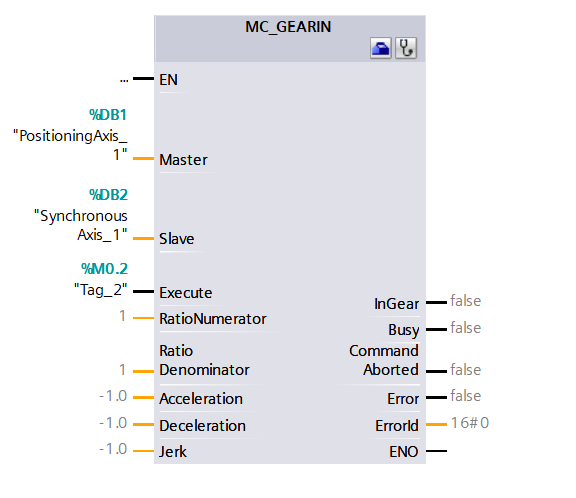
\includegraphics[width = 0.6\textwidth]{Sonne/MC_GearIn.png}    
    \caption{Baustein MC\_GearIn}
    \label{MC_GearIn}
\end{figure}

\subsubsection{Ansteuerung des Förderbands}
\label{Ansteuerung des Förderbandes}
Die Ansteuerung des Förderbands erfolgt im Gegensatz zu den anderen Motoren nicht über Motortreiber. Die Asynchronmaschine des Förderbands wird schlicht und einfach über Relais mit der Spannungsversorgung verbunden oder getrennt. Die Ansteuerung der Relais erfolgt dann über die Digitalausgänge der SPS. Die Relais schalten jeweils die drei Phasen. Eine Richtungsumkehr wird durch eine Vertauschung zweier Phasen erreicht. Deswegen ist das Relais 1 so verschalten, dass das Förderband im Uhrzeigersinn läuft. Beim zweiten Relais sind dann zwei Phasen vertauscht, sodass es zu einer Richtungsumkehr kommt. Dies bedeutet das bei Ansteuern des Relais 1 sich das Förderband im Uhrzeigersinn (+ Richtung ) läuft und beim Ansteuern des  Relais 2 gegen den Uhrzeigersinn (- Richtung). Jedes dieser Relais beistzt auch Hilfskontakte. Diese werden so verkabelt, dass eine Ansteuerung des einen Relais nur geht, sofern das andere Relais nicht angesteurt ist. Dieder Aufbau gleicht einer Wendeschützschaltung. \\
Nun wird bestimmt wie lange man ein Relais ansteuern muss, damit das Förderband eine bestimmte Strecke zurücklegt. Aufgrund des hohen Zeitaufwandes dieses Projektes konnte folgender Ansatz noch nicht umgesetzt werden. Der Ansatz ist es, das Förderband per Direktstart anlaufen zu lassen. Daraufhin wäre die Distanz, die das Förderband nach einer bestimmten Zeit zurücklegt zu messen und mehrere Datenpunkte anzulegen. Beispielsweise bei \qty{0.5}{\second}, \qty{1}{\second}, \qty{2}{\second} und \qty{5}{\second}. Dann wäre eine Regressionsrechnung durchzuführen, um eine Funktion für die zurückgelegte Strecke, in Abhängigkeit von der Zeit zu bekommen. Von dieser Funktion wäre nun eine Umkehrfunktion zu erstellen. Diese liefert dann, die Zeit die es braucht um eine bestimmte Wegstrecke zurückzulegen. Mit dieser Funktion kann dann in Tia Portal gearbeitet werden, in dem man die gewünschte Wegstrecke einsetzt und den zugehörigen Zeitwert bekommt. Dieser Zeitwert ist dann die Zeit, wie lange die Relais angesteuert werden sollen. 

\subsubsection{Tia-Portal Programm}
Durch die SPS-Server Kommunikation stehen die benötigten Daten sowie der Auftrag, welcher ausgeführt werden muss, zu Verfügung. 

    \paragraph{Ein-/Auslagerung} \mbox{} \\
    Bei dieser Aufgabe stehen als Informationen die X,Y,Z -Werte der Lagerposition zu Verfügung und ob es sich um eine Ein- oder Auslagerung handelt. Die Lagerposition ist der linkeste, oberste und vorderste Punkt bei einer Box, wenn diese gelagert ist. Die Tiefe, also der Z-Wert, ist nur wie weit die Z-Achse nach vorne fährt. 
    
    \subparagraph{Einlagerung} \mbox{} \\
    Bei einer Einlagerung muss die Box zuerst beim Querförderer geholt werden. Das Abholen der Box beim Querförderer erfolgt wie die Auslagerung. Dann wird die Box auf die Zielposition gelagert. Die anzufahrenden Wert unterscheiden sich von der Lagerposition. Der anzufahrende X-Wert liegt in der Mitte der Box. 
    \begin{equation*}
        X_{Wert} = X_{Lagerposition} + \frac{Breite der Box}{2}
    \end{equation*}
    Beim Y-Wert wird der Abstandzur Einlagerungsschiene berücksichtigt, welcher aufgrund von Toleranzen sowie der Höhe der Z-Achse, zustande kommt. Dieser Abstand beträgt \qty{30}{\milli\meter}.
    Um nun den X-Wert und Y-Wert, welcher angefahren wird, zu bestimmen, wird folgende Rechnung angewendet:

    \vspace{-6mm}

    \begin{equation*}
        \begin{split}
                X_{Wert} = X_{Lagerposition} + 50
                \\
                Y_{Wert} = Y_{Lagerposition} + 30  
        \end{split} 
    \end{equation*}

    Dann wird der Z-Wert angefahren und die Box anschließend auf:

    \vspace{-6mm}
    \begin{equation*}
        Y_{Wert} = Y_{Lagerposition} - 20
    \end{equation*}

    gesenkt. Dies wird getan um sicherzustellen, dass die Box in der Einlagerungsschiene liegt. \\
    Daraufhin kann die Z-Achse wieder eingefahren werden (Z-Wert = 0). 

    \subparagraph{Auslagerung} \mbox{} \\
    Zuerst die zu auslagernde Box anfahren. 

    \vspace{-6mm}

    \begin{equation*}
        \begin{split}
                X_{Wert} = X_{Lagerposition} + 50
                \\
                Y_{Wert} = Y_{Lagerposition} - 20  
        \end{split} 
    \end{equation*}

    Dann wieder die Z-Achse auf den gegebenen Wert ansteuern und die Box auf:

    \vspace{-6mm}
    \begin{equation*}
        Y_{Wert} = Y_{Lagerposition} + 30
    \end{equation*}
    heben.

    Nun die Box wieder einfahren (Z-Wert = 0). Daraufhin die Position des Querförderes anfahren. Damit wäre der Befehl \enquote{Auslagerung} abgeschlossen.


    \paragraph{Querförderer} \mbox{} \\ 
    Der Querförderer fördert Boxen von Lager auf das Förderband und umgekehrt. Er wird über einen Motor angesteuert. Wenn der Querförderer angesteuert wird, stehen nur die Information zu Verfügung, auf welche Position dieser fahren soll.

    \paragraph{Förderband} \mbox{} \\
    Beim Ansteuern des Förderbands liegen folgende Informationen vor. Zu fahrende Strecke und die Richtung (plus oder minus). Die Richtung wird darüber bestimmt, welches Relais man ansteuert. Relais 1 für plus und Relais 2 für minus. Wie weit nun das Förderband fährt wird über die Einzeit des Relais bestimmt. Die Zeit wie lange das Relais ein sein soll, hängt von der zurückzulegenden Strecke ab. Diese Information steht zu Verfügung, weshalb man diese in die Funktion einsetzt, welche man wie in Punkt \ref{Ansteuerung des Förderbandes} gezeigt ermittelt hat, und bekommt so die Zeit, wie lange das Relais ansteuert wird. Die Bewegung des Förderbands erfolgt immer relativ zur aktuellen Position und nicht absolut. 


    \paragraph{Beispiel für eine solche Ausführung} \mbox{} \\
    Befehle könnten in folgender Reihenfolge kommen:

        \begin{enumerate}
            \item A01 P+1000
            \item A11 P2500
            \item A11 P0000
            \item A10 X0100Y0500Z0250R1
        \end{enumerate}

    Diese werden wie folgt ausgeführt:

        \begin{enumerate}
            \item A01: steht für eine Bewegung des Förderbandes. 
                \subitem +1000 : Eine Bewegung um \qty{1000}{\milli\meter} im Uhrzeigersinn
            \item A11: Ausfahren des Querförderes auf die Position \qty{2500}{\milli\meter} 
            \item A11: Einfahren des Querförderers auf die Position \qty{0}{\milli\meter}
            \item A10: Einlagerung der Box
                \subitem Angesteuert werden dann folgende Werte:

                \vspace{-6mm}
                    \begin{equation*}
                        \begin{split}
                            X_{Wert} = 100 + 50 = 150 \\
                            Y_{Wert} = 500 + 30 = 530 \\
                            Z_{Wert} = 250
                        \end{split}
                    \end{equation*}
                \subitem Die X-Achse und Y-Achse können gleichzeitig auf den   richtigen Wert gefahren werden. Erst wenn die X- und Y-Position erreicht wurde, wird die Z-Achse angesteuert. 
                \subitem Darufhin folgt das Absetzen der Box. Nun wird folgender Y-Wert angefahren:

                \vspace{-6mm}
                    \begin{equation*}
                        \begin{split}
                            Y_{Wert} = 500 - 20 = 480
                        \end{split}
                    \end{equation*}

                \subitem Schlussendlich wird die Z-Achse wieder eingefahren.

                \vspace{-6mm}
                    \begin{equation*}
                        \begin{split}
                            Z_{Wert} = 0
                        \end{split}
                    \end{equation*}
            \item Nun sind alle Aufträge abgeschlossen.
        \end{enumerate}

    Bei diesem Beispielauftrag wurde nicht auf die zeitliche Ausführung geachtet. In welcher Reihenfolge sowie Zeitabstand indem die Befehle kommen, hängt alleine von der Logik am Server ab.

\subsection{SPS-Server Kommunikation}
Da die Lagerlogik auf einem Server ausgeführt wird und die SPS nur das ausführende Element ist, muss eine Verbindung zwischen SPS und Server aufgebaut werden. Das Ziel dieser Verbindung ist es, die nötigen Informationen, sowie die Übertragung des Auftrags auszuführen. 

    \subsubsection{Zur Auswahl stehende Kommunikationsprotokolle} 
    \label{Kommunikationsprotokolle}

    Kommunikationsprotokolle ermöglichen den Datenaustausch zwischen unterschiedlichen Systemen, indem sie Standards und Regeln für die Kommunikation definieren. In diesem Projekt wurden zwei Protokolle getestet und miteinander verglichen: OPC-UA sowie das HTTP-Protokoll.


    \paragraph{Allgemeines}

        \begin{itemize}
            \item \textbf{HTTP (Hypertext Transfer Protocol):}  \mbox{} \\
            HTTP ist eines der bekanntesten Protokolle, welches für die Datenübertragung zwischen Clients und Servern verwendet wird. Es basiert auf einem Anforderungs-Antwort-Prinzip, bei dem ein Client (Bsp.: Webbrowser) Anfragen an einen Server sendet, welcher anschließend die entsprechenden Daten zurückschickt. Die Anfrage wird als HTTP Request und die Antwort als HTTP Response bezeichnet.(vgl. \cite{HTTP-Allgemein})
            
            \item \textbf{OPC-UA (Open Platform Communications - Unified Architecture):} \mbox{} \\
            OPC-UA (Open Platform Communications Unified Architecture) ist ein plattformunabhängiges Kommunikationsprotokoll, das speziell für industrielle Anwendungen entwickelt wurde. Es ermöglicht eine herstellerunabhängige Kommunikation zwischen verschiedenen Geräten bzw. Systemen. (vgl. \cite{OPC-UA})
        \end{itemize}

    \paragraph{Funktionsweise}

            \begin{itemize}
                \item \textbf{{HTTP (Hypertext Transfer Protocol):}} \mbox{} \\
                Eine Kommunikation mit dem HTTP Protokoll findet wie folgt statt. Wie oben bereits erwähnt funktioniert das HTTP- Protokoll nach dem Anforderungs-Antwort-Prinzip. Wie in Abb. \ref{HTTP-Client_Server_Kommunikation} ersichtlich wir als Erstes eine Anfrage vom Client zum Server gesendet (HTTP-Request). Darufhin wird diese Anfrage vom Server bearbeitet und dieser sendet dann die geforderten Informationen zurück (HTTP-Response). Danach ist die Verbindung beendet.
                (vgl. \cite{HTTP-Client_Server_Kommunikation})

                \begin{figure}[h]
                    \centering
                    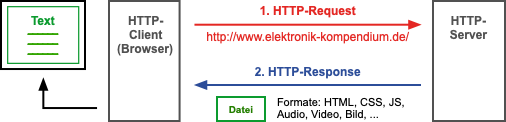
\includegraphics[width = 0.8\textwidth]{Sonne/HTTP-Client_Server_Kommunikation.jpg}
                    \caption{HTTP-Client-Server Kommunikation, Quelle:  
                    \cite{HTTP-Client_Server_Kommunikation}}
                    \label{HTTP-Client_Server_Kommunikation}
                \end{figure}
            
                \item \textbf{{OPC-UA (Open Platform Communications - Unified Architecture):}} \mbox{} \\
                Auch bei OPC UA gibt es Server und Clients. Dabei stellt der Server Daten bereit und die Clients können diese Daten abfragen oder Werte überschreiben. Dies ermöglicht einen sichere sowie zuverlässige Datenübertragung. 
                (vgl. \cite{OPC-UA})
            \end{itemize}

            
    \paragraph{Auswahl des Protokolls} \mbox{} \\
    Bei diesem Projekt wurde das HTTP Protokoll ausgewählt, um die Kommunikation zwischen SPS und Server auszuführen. Das HTTP Protokoll wurde ausgewählt, da die SPS direkt mit dem Server kommunizieren kann. Bei OPC-UA hätte ein zusätzlicher Server gehostet werden müssen. Dieser OPC-UA Server hätte dann mit dem eigentlichen Server, welcher die Lagerlogik übernimmt, kommuniziert. Die SPS hätte dann auf den OPC-UA Server zugegriffen und nicht direkt auf den Zielserver. Um diesen zusätzlichen Aufwand sowie weitere Fehlerquellen zu vermeiden, wurde das HTTP Protokoll ausgewählt.
            
            

    
    \subsubsection{Verbindungsherstellung}
    Aus den in Punkt \ref{Kommunikationsprotokolle} genannten Gründen wurde das HTTP Protokoll ausgewählt. Um in TIA-Portal die Verbindung via HTTP aufzubauen, benötigt man bestimmte Libraries die von Siemens zu Verfügung gestellt werden. Diese müssen dann wie im Punkt \ref{Bilbliotheken} gezeigt eingebunden werden, um die Funktionsbausteine der Library nutzen zu können. 

        \paragraph{Funktionsbausteine} \mbox{} \\
        In der Library für das HTTP Protokoll stehen dann folgende Bausteine zur Verfügung:

        \begin{itemize}
            \item GET
            \item POST-PUT 
        \end{itemize}
    
    Als Baustein zur Verbindungsherstellung wurde der POST-Befehl ausgewählt, da mit diesem unbegränzte Datenmengen geschickt werden können. Damit der Baustein nun eine Verbindung herstellen kann müssen folgende Parameter angegeben werden: \textbf{URL} [string], die zu schickenden Daten \textbf{data} [string] und ein Speicherplatz für die empfangenen Daten \textbf{response Data} [Array of Char]. Die restlichen Eingabeparameter, welche in Abb. \ref{POST-PUT_Baustein} ersichtlich sind,  müssen nicht unbedingt ausgefüllt werden, sondern werden automatisch vorausgefüllt. Standardmäßig ist die richtige Methode (POST) schon ausgewählt, da die Eingabe \textbf{method} automatisch mit \textbf{0} ausgefüllt wird. 

    \begin{figure} [h]
        \centering
        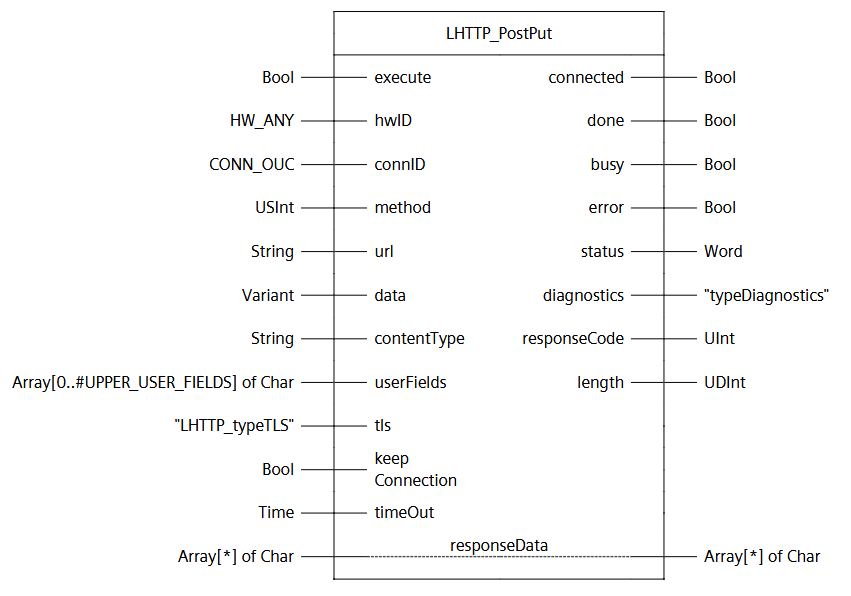
\includegraphics[width = 0.7\textwidth] {Sonne/POST-PUT_Baustein.png}
        \caption{POST-Put  Baustein, Quelle: \cite{HTTP-Bausteine}}
        \label{POST-PUT_Baustein}
    \end{figure}

    Wird nun die Eingabe \textbf{execute} HIGH, so wird der Baustein einmalig ausgeführt. Rechnet man mit einem häufigeren Datenaustausch, mit Hilfe dieses Bausteins, so empfiehlt es sich den Parameter \textbf{keep Connenction} auf \textbf{true} zu setzen. Dadurch bleibt die Verbindung mit dem Zielserver erhalten und weitere Kommunikationen werden schneller ausgeführt. 

    \subsubsection{Datenaustausch}
    \label{Datenaustausch}
    Die SPS und der Server arbeiten mit verschiedenen Datentypen. Bei dem Datenaustauch erwartet der Server die Daten in einem json-Format. Deswegen müssen die Daten, welche gesendet werden, zuerst in dieses Format gebracht werden. Um dies in Tia Portal zu realisieren wird die Bibilothek LStream eingebunden. Mit dieser werden dann Daten aus einem json-Datenbaum in ein Array of Byte umgewandelt. Dieses Array of Byte wird anschließend in den Datentyp string umgewandelt. Nun kann dieser string an den POST-Datenbaustein weitergegeben werden. \\
    Ist nun der Datenaustauch abgeschlossen, so sind die empfangenen Daten als Array of Char verfügbar. Da man in Tia-Portal nur umständlich mit diesem Datenformat umgehen kann, wird das Array of Char nun in das Datenformat string umgewandelt. Die Daten sind nun noch immer nicht einzeln verfügbar, weswegen man nun diesen string nach den Daten filtern muss.

    \subsubsection{Datenfilterung}
    Die vom Server geschickten Daten werden in einem Befehl geschickt. Aus diesem Befehl muss herausgelesen werden, um welche Aufgabe es sich handelt  und welche Daten erforderlich sind, um diese Aufgabe auszuführen.

        \paragraph{Datenformatierung}\mbox{}\\
        Die Daten werden in einem string geschickt, welcher in zwei Teile aufgeteilt wird. Der zweite Teil ist jedoch abhängig vom ersten. \\
        (In folgenden Punkten dient x immer als Platzhalter für eine Nummer null bis neun.) 
        \begin{itemize}
            \item 1.Teil: \\
            IDxxxxAxx  \\
            Aus diesem Teil werden die ID-Nummer sowie der Auftrag herausgefiltert. Die ID-Nummer ist eine 4 stellige Nummer welche nach ID steht. Der auszuführende Teil der Hardware steht in den zwei Stellen nach A.\\
            Diese werden nach folgender Codierung ausgelesen:
                \subitem 00: Kommissionierstation
                \subitem 01: Förderband
                \subitem 10: Lager 1 (Aus-/Einlagerung)
                \subitem 11: Lager 1 (Querförderer)
            \item 2.Teil: \\
            Der zweite Teil steht in Abhängigkeit zum Ersten. Je nachdem welche Zahl nach A steht, also der Code welche Area angesprochen wird, ist der zweite Teil anders aufgebaut.
                \begin{itemize}
                \item 00: SB\\
                Bei diesem Befehl muss der Barcodescanner angesteuert werden um an der Kommissionierstation einen Barcode einzuscannen.
                \item 01: P $\pm$xxxx \\
                Gibt an um wie viel sich das Förderband (in mm) bewegen muss. Vor der Zahl steht jedoch entweder ein plus oder minus um festzulegen, in welche Richtung sich das Förderband bewegen muss. 
                \item 10: XxxxxYxxxxZxxxxRx \\
                Nach jeder Achse X,Y,Z steht ein vierstelliger Wert, der die Position des gewünschten Lagerplatzes angibt. Der Wert nach R ist entweder 0 oder 1 und gibt an ob es sich um eine Einlagerung (1) oder Auslagerung (0) handet.
                \item 11: Pxxxx \\
                Nach P steht ebenso ein vierstelliger Wert, der angibt auf welche Position der Querförderer gefahren werden muss. 
                
                \end{itemize}
            
        \end{itemize}

    \subsubsection{Tia Portal Programm}
    Im Programm werden zwei Funktionsbausteine aufgerufen. Nämlich FB\_Kommunikation und FB\_Datenfiltern. FB\_Kommunikation übernimmt den Datenaustausch zwischen Server und SPS. In diesem Baustein werden zuerst die Daten die an den Server geschickt werden, wie in Punkt \ref{Datenaustausch} erklärt, ins richtige Datenformat (string) gebracht. Darufhin wird der HTTP POST-Aufruf ausgeführt und die empfangenen Daten, wie in \ref{Datenaustausch} gezeigt, wieder ins richtige Datenformat gebracht. Somit ist die Aufgabe dieses Datenbausteins erfüllt. Nun erfolgt der Aufruf des zweiten Funktionsbausteins FB\_Datenfiltern. Dieser Funktionsbaustein ist in unterschiedliche Funktionsbausteine aufgeteilt. Der erste dieser Funktionsbausteine filtert nach ID sowie der Area (Aufgabe). Daraufhin wird der Baustein FB\_Kommunikation innerhalb des Bausteins FB\_Datenfiltern aufgerufen, um sofort die ID-Nummer an den Server zurück zu schicken, damit dieser weiß, dass die SPS den Auftrag erhalten hat. Die restlichen Bausteine die im FB\_Datenfiltern enthalten sind, warten darauf, dass sie von ihrer Area, beispielsweise 01, angesprochen werden. Sollte dies der Fall sein, so filtern sie die für den Auftrag benötigten Informationen. Nach dem Aufruf beider Bausteine sind nun die geforderten Informationen verfügbar. Bei beiden Funktionsbausteinen handelt es sich um Multiinstanzen, um das Programm übersichtlicher zu halten. 

    \paragraph{SCL-Bausteine (am Beispiel \enquote{ID + Area})} 
    \mbox{} \\
    Alle Bausteine zur Datenfilterung wurden in SCL programmiert. Als Eingabe dient der string, welcher die Daten beinhaltet. In diesem wird zuerst nach ID gefiltert (siehe Code-Snippet \ref{SCL-Baustein}, Zeile 1). Dies liefert die Position von ID innerhalb des Strings. Daraufhin werden alle Zeichen links von ID + ID wegelöscht (siehe Code-Snippet \ref{SCL-Baustein}, Zeilen 2 bis 5). Nun weiß man das rechts von ID eine vierstellige Nummer (ID-Nummer) steht. Da alles links von dieser Nummer weggeschnitten wurde, weiß man das diese Nummer ganz links im string ist. Deswegen werden die ersten vier Stellen von links genommen und dem Ausgang Q\_Info\_ID zugewiesen (siehe Code-Snippet \ref{SCL-Baustein}, Zeile 6). Dieser Ausgang ist für das gesamte Programm erreichbar. Dasselbe Suchen und Löschen der Zeichen links vom Gesuchten wird ebenfalls für A (Area / Auftrag) erledigt (siehe Code-Snippet \ref{SCL-Baustein}, Zeilen 10 bis 13). Da man den Wert von Area, welcher den Auftrag definiert, vergleichen will um den richtigen Baustein auszuführen, werden die zwei Zeichen links von A, von denen wir wissen das es Zahlen sind, in das Datenformat int konvertiert und dem Ein-Ausgang IQ\_Info\_Area zugewiesen (siehe Code-Snippet \ref{SCL-Baustein}, Zeilen 19 bis 23). \\

    \begin{lstlisting}[language=Pascal, caption={SCL Baustein \enquote{ID+Area}}, label = SCL-Baustein]
        #T_Int := FIND(IN1 := #I_Datenstring, IN2 := 'ID');
IF #T_Int > 0 THEN
    #X_Info_ID := #T_Int + 1;
    #X_String_bearbeitet := DELETE(IN := #I_Datenstring, L := #X_Info_ID, P := 1); //Alles bis inkl. X wegschneiden
    
    #Q_Info_ID := LEFT(IN := #X_String_bearbeitet, L := 4);               // 4 Zeichen links von X nehmen
    
END_IF;

#T_Int := FIND(IN1 := #I_Datenstring, IN2 := 'A');
IF #T_Int > 0 THEN
    #X_Info_Area := #T_Int + 0;
    #X_String_bearbeitet := DELETE(IN := #I_Datenstring, L := #X_Info_Area, P := 1);
    
    // Lager herausfinden                      10: Lager 1      11: Puscher (Lager 1)       00: Komissionierstation
    //(zurzeit nur 1 Lager verfuegbar)          20: Lager 2      21: Puscher (Lager 2)       01: Foerderband
    // -->nur 00/01/10/11 relevant             30: Lager 3      31: Puscher (Lager 3)
    
    #Area_Info_1_string := LEFT(IN := #X_String_bearbeitet, L := 2);
    STRG_VAL(IN := #Area_Info_1_string,                                         
             FORMAT := #Area_convert_Format_auswaehlen,
             P := 1,
             OUT => #IQ_Info_Area);
    
END_IF;
    \end{lstlisting}


\subsection{Herausforderungen}
